%% LyX 2.0.4 created this file.  For more info, see http://www.lyx.org/.
%% Do not edit unless you really know what you are doing.
\documentclass[submission,copyright,creativecommons]{eptcs}
\usepackage{courier}
\usepackage[latin9]{inputenc}
\setcounter{secnumdepth}{3}
\setcounter{tocdepth}{3}
\usepackage{url}
\usepackage{graphicx}

\makeatletter

%%%%%%%%%%%%%%%%%%%%%%%%%%%%%% LyX specific LaTeX commands.
%% Because html converters don't know tabularnewline
\providecommand{\tabularnewline}{\\}

%%%%%%%%%%%%%%%%%%%%%%%%%%%%%% User specified LaTeX commands.

\providecommand{\event}{TTC 2013} 

\def\titlerunning{Petri Nets to Statecharts}
\def\authorrunning{P. {Van Gorp} and L.M. Rose}

\usepackage{url}\usepackage{color}\usepackage{listings}


\title{The Petri-Nets to Statecharts Transformation Case}

\author{Pieter Van Gorp \institute{Eindhoven University of Technology, PO Box 513, 5600 MB Eindhoven, The Netherlands.} \email{p.m.e.v.gorp@tue.nl} \and Louis M. Rose \institute{Department of Computer Science, University of York, UK.} \email{louis.rose@york.ac.uk}}

\makeatother

\begin{document}
\maketitle

TODO: 
\begin{itemize}
\item Abstract 
\item Nice healthcare example
\item Describe the huge models for stresstesting
\item Cite MODELS paper for the results of Java, GrGen, and mention that
Epsilon is X times slower for now. 
\item Evaluation criteria: table
\item Elaborate text for bonus features
\item Create ZIP attachment with testsuite models
\end{itemize}

\section{Introduction}

Although transformations are already developed for decades in various
communities (such as the compiler community~\cite{Bacon1994compilertrans},
the program transformation community~\cite{Feather87progtranssurv}
and the business process management (BPM) community~\cite{Lohmann09BPMtransSurv}),
it is relatively new to study the strengths and weaknesses from transformation
approaches across community boundaries. The aim of the Transformation
Tool Contest (TTC) is to compare the expressiveness, the usability
and the performance of graph and model transformation tools along
a number of selected case studies. A deeper understanding of the relative
merits of different tool features will help to further improve graph
and model transformation tools and to indicate open problems~\cite{TTC11Proceedings}.
This paper proposes a case for the sixth edition of TTC (i.e., to
TTC'13).


\subsection{Context of the Case}

In BPM research and practice, transformations are usually programmed
using general purpose programming languages. Mapping rules in BPM
literature tend to be formalized using mathematical set constructs
whereas they tend to be documented using informal visual rules and
implemented in Java or another general purpose programming language.
In the graph and model transformation communities, special purpose
languages and tools are being developed to support the direct execution
of such mapping rules. Finally, various comparative studies have been
contributed to the emerging field of transformation engineering (cfr.,~\cite{Taentzer2005_ModelTransformationsbyGraphTransformationsAComparativeStudy,Varro2008_TransformationofUMLModelstoCSPACaseStudyforGraphTransformationTools,Rensink2010_Graphtransformationtoolcontest2008,Gronmo2009_ComparisonofThreeModelTransformationLanguages,Rose2009_AnAnalysisofApproachestoModelMigration,rose10comparison,vAmstel2011ATLQVTperfAnal,Tolosa2011TSMatlMeasurement})
but too little transformation problems have been considered that are
considered challenging by the BPM community. This paper proposes the
so-called PN2SC case, related to the transformation of Petri-Nets
to statecharts. The case relates to an active research line at Eindhoven
University of Technology. Interestingly, much of the associated research
efforts have been spent on an optimization algorithm which turns out
to be irrelevant when using a rule-based transformation approach instead
of an imperative programming approach~\cite{VanGorp2010MoDELS}.
Therefore, the case can be considered a nice showcase for demonstrating
to the BPM community the potential impact of results from the transformation
community.


\subsection{Relevance for TTC'13}

Besides providing %interesting
input to BPM industry and its research community, this study also
covers a previously unstudied type of transformation. More specifically,
the transformation problem under study is a process model translation
that raises the abstraction level. Regardless of concrete language
and metamodel details, this type of problem has not yet been considered
for the evaluation of transformation approaches. 

In the following, we briefly survey existing comparative studies related
to process models. Varr� et al. studied various approaches to mapping
conceptual process model in UML to more technical CSP models~ \cite{Varro2008_TransformationofUMLModelstoCSPACaseStudyforGraphTransformationTools}.
Also, in a special issue edited by Rensink et al., various experts
present their solutions to a case study concerning the mapping of
conceptual process models in BPMN to more technical BPEL models~\cite{Rensink2010_Graphtransformationtoolcontest2008}.
Gr�nmo et al. discuss various approaches to transforming conceptual
UML models into strictly structured counter-parts~\cite{Gronmo2009_ComparisonofThreeModelTransformationLanguages}.
Again, the target models are more low-level than the input models.
Rose et al. discuss different approaches to migrating Petri-Net models~\cite{rose10comparison}.
In that case, input models are at the same level of abstraction as
output models. 

Van Gorp et al. have already considered the case proposed by this
paper for comparing a graph transformation approach to the Java-based
programming approach that is mainstream in the BPM domain. The authors
make the interesting observation that the rule-based approach required
less specification efort yet delivered superior performance. By submitting
this case to TTC'13, we aim at analyzing the generalizability of that
observation.


\subsection{Input and Output Languages}

TODO: copy/paste some background about petri-nets and statecharts,
also cite some papers about safe nest, workflow nets.


\section{The Transformation}

This section details the Petri-Net to statechart transformation algorithm,
originally described by Eshuis \cite{eshuis09translating}. The transformation
described below is \emph{input-destructive} (elements of the Petri-Net
model are removed as the transformation proceeds), and uses the metamodels
shown in figure~\ref{fig:mms}.

\begin{figure}[tb]
\centerline{ %
\begin{tabular}{c||c}
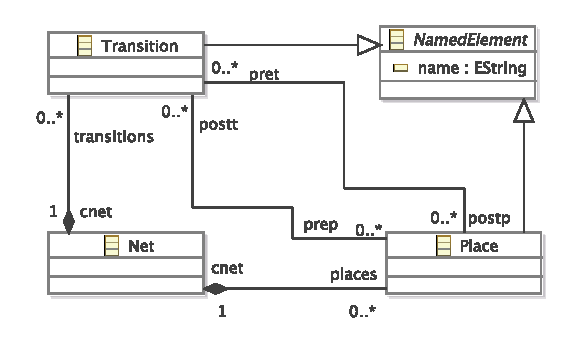
\includegraphics[width=0.45\linewidth]{images/PetriNets}  & 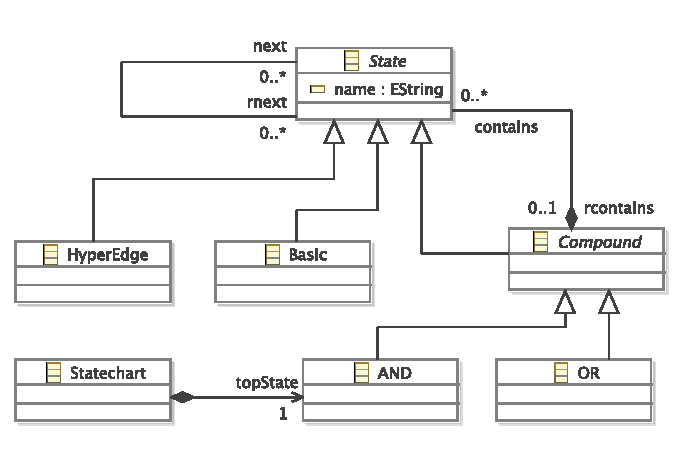
\includegraphics[width=0.5\linewidth]{images/StateCharts}\tabularnewline
(a) Petri-Net metamodel  & (b) Statechart metamodel \tabularnewline
\end{tabular}} \caption{\label{fig:mms}The metamodels used in the PN2SC transformation.}
\end{figure}



\subsection{Preconditions}

The following assumptions can be made regarding the context in which
the PN2SC transformation is started: 
\begin{itemize}
\item there is only one instance of \texttt{Net},
\item there are no \texttt{Statechart} nor \texttt{State} instances.
\end{itemize}

\subsection{Initialisation}

The first step in the PN2SC transformation involves creating an initial
structure for the statechart model. In particular, the following statechart
model elements are created:
\begin{itemize}
\item For every \texttt{Place} $p$ in the Petri-Net: \subitem an instance
of \texttt{Basic}, $b$ (with $b.name=p.name$), \subitem an instance
of \texttt{OR}, $o$ such that $o.contains=\{b\}$,
\item For every \texttt{Transition} $t$ in the Petri-Net: \subitem an
instance of \texttt{HyperEdge} $e$ (with $e.name=t.name$),
\item All \texttt{pret/postp} and \texttt{postt/prep }arcs should be mapped
to \texttt{next/rnext} links between the \texttt{States} equivalent
with the input \texttt{NamedElements} that are connected by these
arcs.
\end{itemize}

\paragraph{Equivalence.}

Initialisation should also provide a mechanism for identifying the
\texttt{OR} node created for a particular \texttt{Place} and the \texttt{HyperEdge}
created for a particular \texttt{Transition}. The precise mechanism
can vary over implementations. One approach is to use a name-based
identification (e.g., assign all \texttt{Places} a uniquely identifying
name and copy each \texttt{Place's} name to its \texttt{OR} node during
initialisation.) Another approach is to create traceability links
between corresponding source and target elements. In the remainder
of this section we assume that the initialisation of the transformation
will construct an injective function $equiv:Place\to OR$.


\subsection{Reduction rules}

Following initialisation, the transformation continues by applying
one of two types of reduction rules: AND and OR. 

\begin{figure}[tb]
\centerline{ %
\begin{tabular}{c||c}
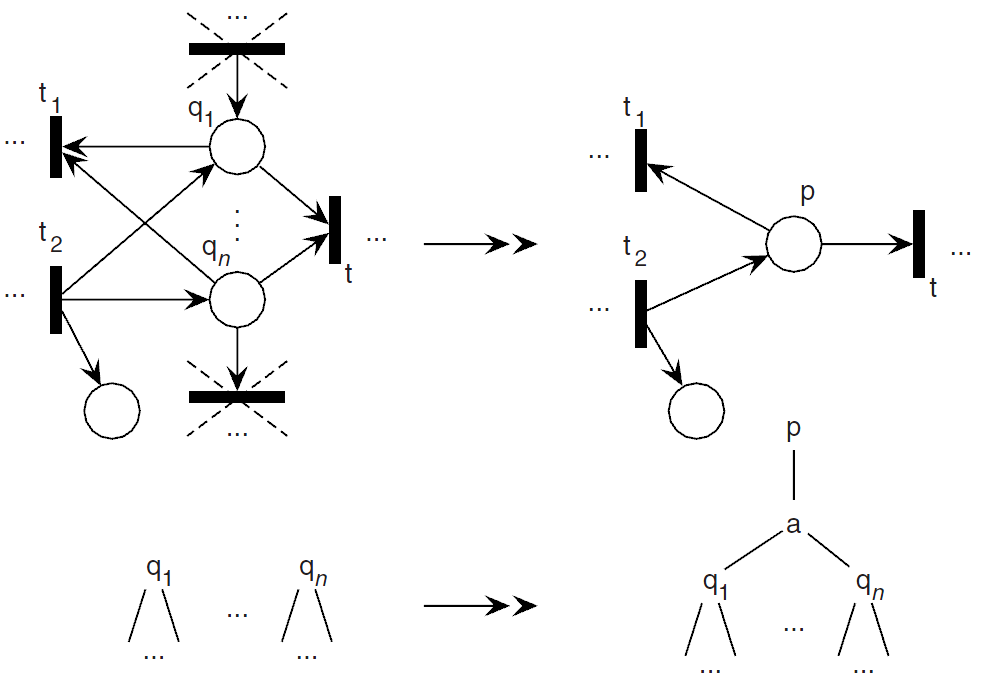
\includegraphics[width=0.45\linewidth]{images/figs-R1a}  & 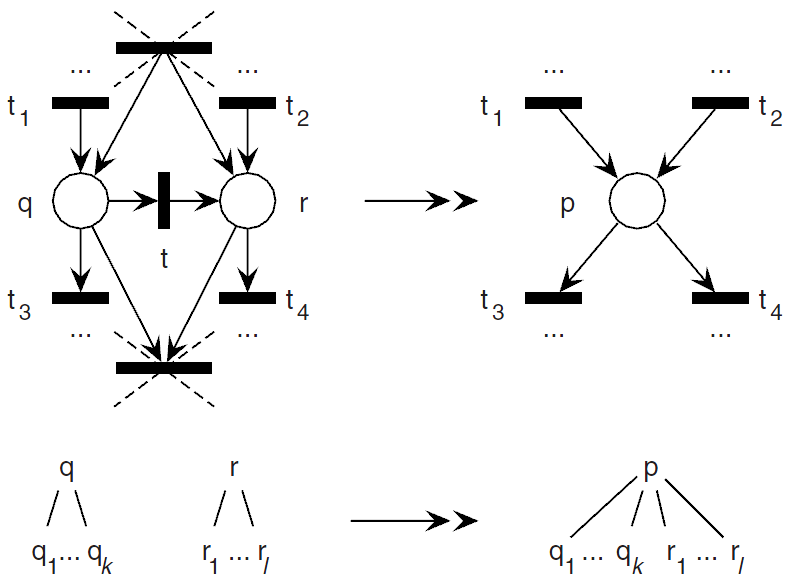
\includegraphics[width=0.5\linewidth]{images/figs-R2}\tabularnewline
(a) rule for creating \emph{AND nodes}  & (b) rule for merging \emph{OR nodes}\tabularnewline
\end{tabular}} \caption{\label{fig:Visual-documentation-for-rules}Visual documentation for
mapping rules.}
\end{figure}



\subsubsection{AND rules}

The first type of reduction rule, AND (informally documented by Figure~\ref{fig:Visual-documentation-for-rules}.a),
constructs an \texttt{AND} state for a set of \texttt{Places} that
are connected to the same incoming and outgoing \texttt{Transitions}.


\paragraph{Pre-conditions.}

The AND rule can be applied to a \texttt{Transition}, $t$, iff $\left|t.prep\right|>1$
and every \texttt{Place} in $t.prep$ is connected to the same set
of outgoing transitions and the same set of incoming transitions.
Alternatively, the AND rule can be applied to a \texttt{Transition},
$t$ iff $\left|t.postp\right|>1$ and every \texttt{Place} in $t.postp$
is connected to the same set of outgoing transitions and the same
set of incoming transitions. Given these two alternative situations,
we refer to two AND rules. However, in some languages one can implement
these variants in one rule.

Figure~\ref{fig:Visual-documentation-for-rules}.a illustrates when
the AND rule for the situation $\left|t.prep\right|>1$ would be applicable:
$q_{1}$ to $q_{n}$ all have $\{t$\} as the set of outgoing transitions
while they share $\{t_{1},t_{2}\}$ as the set of incoming transitions.
$q_{n}$ should not have an outgoing arc to a transition for which
there is no corresponding arc between $q_{1}$ and that transition.
Conversely, $q_{1}$ should not have an incoming arc from a transition
for which there is no corresponding arc between that transition and
$q_{n}$. To illustrate the situation when the AND rule for the situation
$\left|t.postp\right|>1$ would be applicable, one can simply reverse
all arcs in Figure~\ref{fig:Visual-documentation-for-rules}.a.


\paragraph{Effect on statechart.}

Applying the AND rule results in the creation of a new \texttt{AND}
state ($a$) and a new \texttt{OR} state ($p$) such that $p.contains={a}$
and $a.contains$ is the set of \texttt{OR} states $\{q\in t.prep:equiv(q)\}$;
or $\{q\in t.postp:equiv(q)\}$ if the rule has been applied to the
transition's postset, $t.postp$.


\paragraph{Effect on Petri-Net.}

Applying the AND rule removes from the Petri-Net all but one of the
\texttt{Places} in the set $t.prep$ ($t.postp$).


\paragraph{EOL Implementation.}

Figure~\ref{fig:eol-merge-and} shows an implementation of the AND
rule in EOL. Note that the AND rule can be applied in ``both directions''
on line 2.

\begin{figure}
{\tiny \lstset{escapeinside={(*@}{@*)}}

\definecolor{gray}{rgb}{0.5,0.5,0.5}
\lstset{numbers=left,numbersep=3pt,numberstyle=\tiny,stringstyle={\color{gray}},basicstyle=\tiny,breaklines=true,emph={while,var,false,true,new,for,if,break,not,and,or,operation,Boolean,return, delete,self},emphstyle=\textbf,morecomment=[l][\color{gray}\textit]{//},morestring=[b]",showstringspaces=false,tabsize=2}
\tt
\begin{lstlisting}
operation PN!Transition apply_and_rule() : Boolean {
	return self.apply_and_rule(self.prep) or self.apply_and_rule(self.postp);
}

operation PN!Transition apply_and_rule(places : Collection(PN!Place)) : Boolean {
	var result = false;
	
	// Check pre-conditions
	if (places.size() > 1 and places.forAll(p|p.has_same_transitions_as?(places.first))) {
	  
	  // Alter statechart
		var parent = new SC!AND;
		parent.contains.addAll(places.equivalent());
		
		var root = new SC!OR;
		get_top_state().contains.add(root);		
		root.contains.add(parent);
		
		// Alter Petri net
		delete places.tail();
		
		result = true;
	}
	
	return result;
}

operation PN!Place has_same_transitions_as?(other : PN!Place) : Boolean {
	return self.pret.size() == other.pret.size() and
	       self.postt.size() == other.postt.size() and
	       self.pret.forAll(e|other.pret.includes(e)) and
	       self.postt.forAll(e|other.postt.includes(e));
}

operation Collection tail() : Collection {
	var tailed = self.clone();
	tailed.removeAt(0);
	return tailed;
}

operation PN!Place equivalent() : SC!OR {
	// This operation is implementation-specific.
	// In our solution, we use the names of Places and OR
	// nodes to implement equivalence, but other approaches
	// are equally valid and correct.
}
\end{lstlisting}}{\tiny \par}

\caption{\label{fig:eol-merge-and}EOL code for performing AND merges (Figure~\ref{fig:Visual-documentation-for-rules}a).}
\end{figure}



\subsubsection{OR rules}

The second type of reduction rule, OR (informally documented by Figure~\ref{fig:Visual-documentation-for-rules}.b),
constructs an \texttt{OR} state for a \texttt{Transition} that has
a single preceding \texttt{Place} and single succeeding \texttt{Place}.


\paragraph{Pre-conditions.}

The OR rule can be applied to a \texttt{Transition}, $t$, iff $(\left|t.prep\right|=1)\land(\left|t.postp\right|=1)$
and there is no transition, $t'$, such that $(q\in t'.prep)\land(r\in t'.prep)$
or $(q\in t'.postp)\land(r\in t'.postp)$ where $q$ is the single
place contained in $t.prep$ and $r$ is the single place contained
in $t.postp$.


\paragraph{Effect on statechart.}

Applying the OR rule results in the creation of a new \texttt{OR}
state ($p$) such that $p.contains$ is the set of \texttt{OR} states
$equiv(q).contains\cup equiv(r).contains$.


\paragraph{Effect on Petri-Net.}

Applying the OR rule removes from the Petri-Net the \texttt{Transition}
$t$ and the \texttt{Places} $q$ and $r$; and adds a new \texttt{Place}
$p$ such that $p.pret=(q.pret\cup r.pret)$ and $p.postt=(q.postt\cup r.postt)$.


\paragraph{EOL Implementation.}

Figure~\ref{fig:eol-merge-or} shows an implementation of the OR
rule in EOL. Note that this implementation re-uses $q$ to form $p$,
rather than instantiate a new \texttt{Place} or \texttt{OR} state.

\begin{figure}
\lstset{escapeinside={(*@}{@*)}}

\definecolor{gray}{rgb}{0.5,0.5,0.5}
\lstset{numbers=left,numbersep=3pt,numberstyle=\tiny,stringstyle={\color{gray}},basicstyle=\tiny,breaklines=true,emph={while,var,false,true,new,for,if,break,not,and,or,operation,Boolean,return, delete,self},emphstyle=\textbf,morecomment=[l][\color{gray}\textit]{//},morestring=[b]",showstringspaces=false,tabsize=2}
\tt
\begin{lstlisting}
operation Transition apply_or_rule() : Boolean {
	var result = false;
	
	if (self.prep.size() == 1 and self.postp.size() == 1) {
		var q = self.prep.first;
		var r = self.postp.first;
	
		if ((q == r) or not q.shares_a_transition_with?(r)) {		
			if (q <> r) {
			  var merger = q.equivalent();
  			var mergee = r.equivalent();
  			
				// Update statechart, re-using the q state as p
				merger.contains.addAll(mergee.contains);	
				delete mergee;
				
				// Update Petri net, re-using the q place as p
				q.pret.addAll(r.pret);
				q.postt.addAll(r.postt);
				delete r;
				delete self;
				
				result = true;
			}
		}
	}

	return result;
}

operation Place shares_a_transition_with?(other : Place) : Boolean {
	return self.pret.exists(e|e.postp.includes(other)) or 
	       self.postt.exists(e|e.prep.includes(other));
}

\end{lstlisting}

\caption{\label{fig:eol-merge-or}EOL code for performing OR merges (Figure~\ref{fig:Visual-documentation-for-rules}b).}
\end{figure}



\subsection{Termination}

The output model should contain a single instance of \texttt{Statechart}
$sc$. The transformation should apply the reduction rules as long
as possible to the input elements. For input Petri-Nets in the class
of safe nets, the reduction process should terminate with exactly
one \texttt{Place} left. The equivalent \texttt{AND} state $st$ should
not have any parent \texttt{Compound} state. Moverover, $sc.topState=st$
should hold for $sc$. For unsafe input nets, the reduction rules
typically cannot produce a unique top-level \texttt{AND} state so
it is impossible to produce a model that conforms strictly to the
output model. However, in that case the transformation should terminate
in a state that can only be reached after sequentially applying the
reduction rules as long as possible. It should be possible to inspect
the resulting state of the input Petri-Net for further analysis purposes.


\section{Example Transformation Execution Trace}

This section demonstrates the intended behavior of the reduction rules
from the previous section. Figure~\ref{fig:Visualization-ANDandOR}
visualizes an execution trace for an input model with 11 places and
10 transitions. The input Petri-Net model is shown on the left of
the figure while its corresponding statechart is shown at the right
of the figure. Places are represented as white circles and transitions
as black bars. Basic states are represented as yellow ovals while
hyperedges are represented as black bars too. OR states are represented
as white boxes while AND states are represented as gray boxes. The
top of the figure shows an execution snapshot after initialization.
Each \texttt{Place} and \texttt{Transition} element has respectively
its corresponding \texttt{Basic} state and \texttt{HyperEdge}. 

\begin{figure}


\begin{centering}
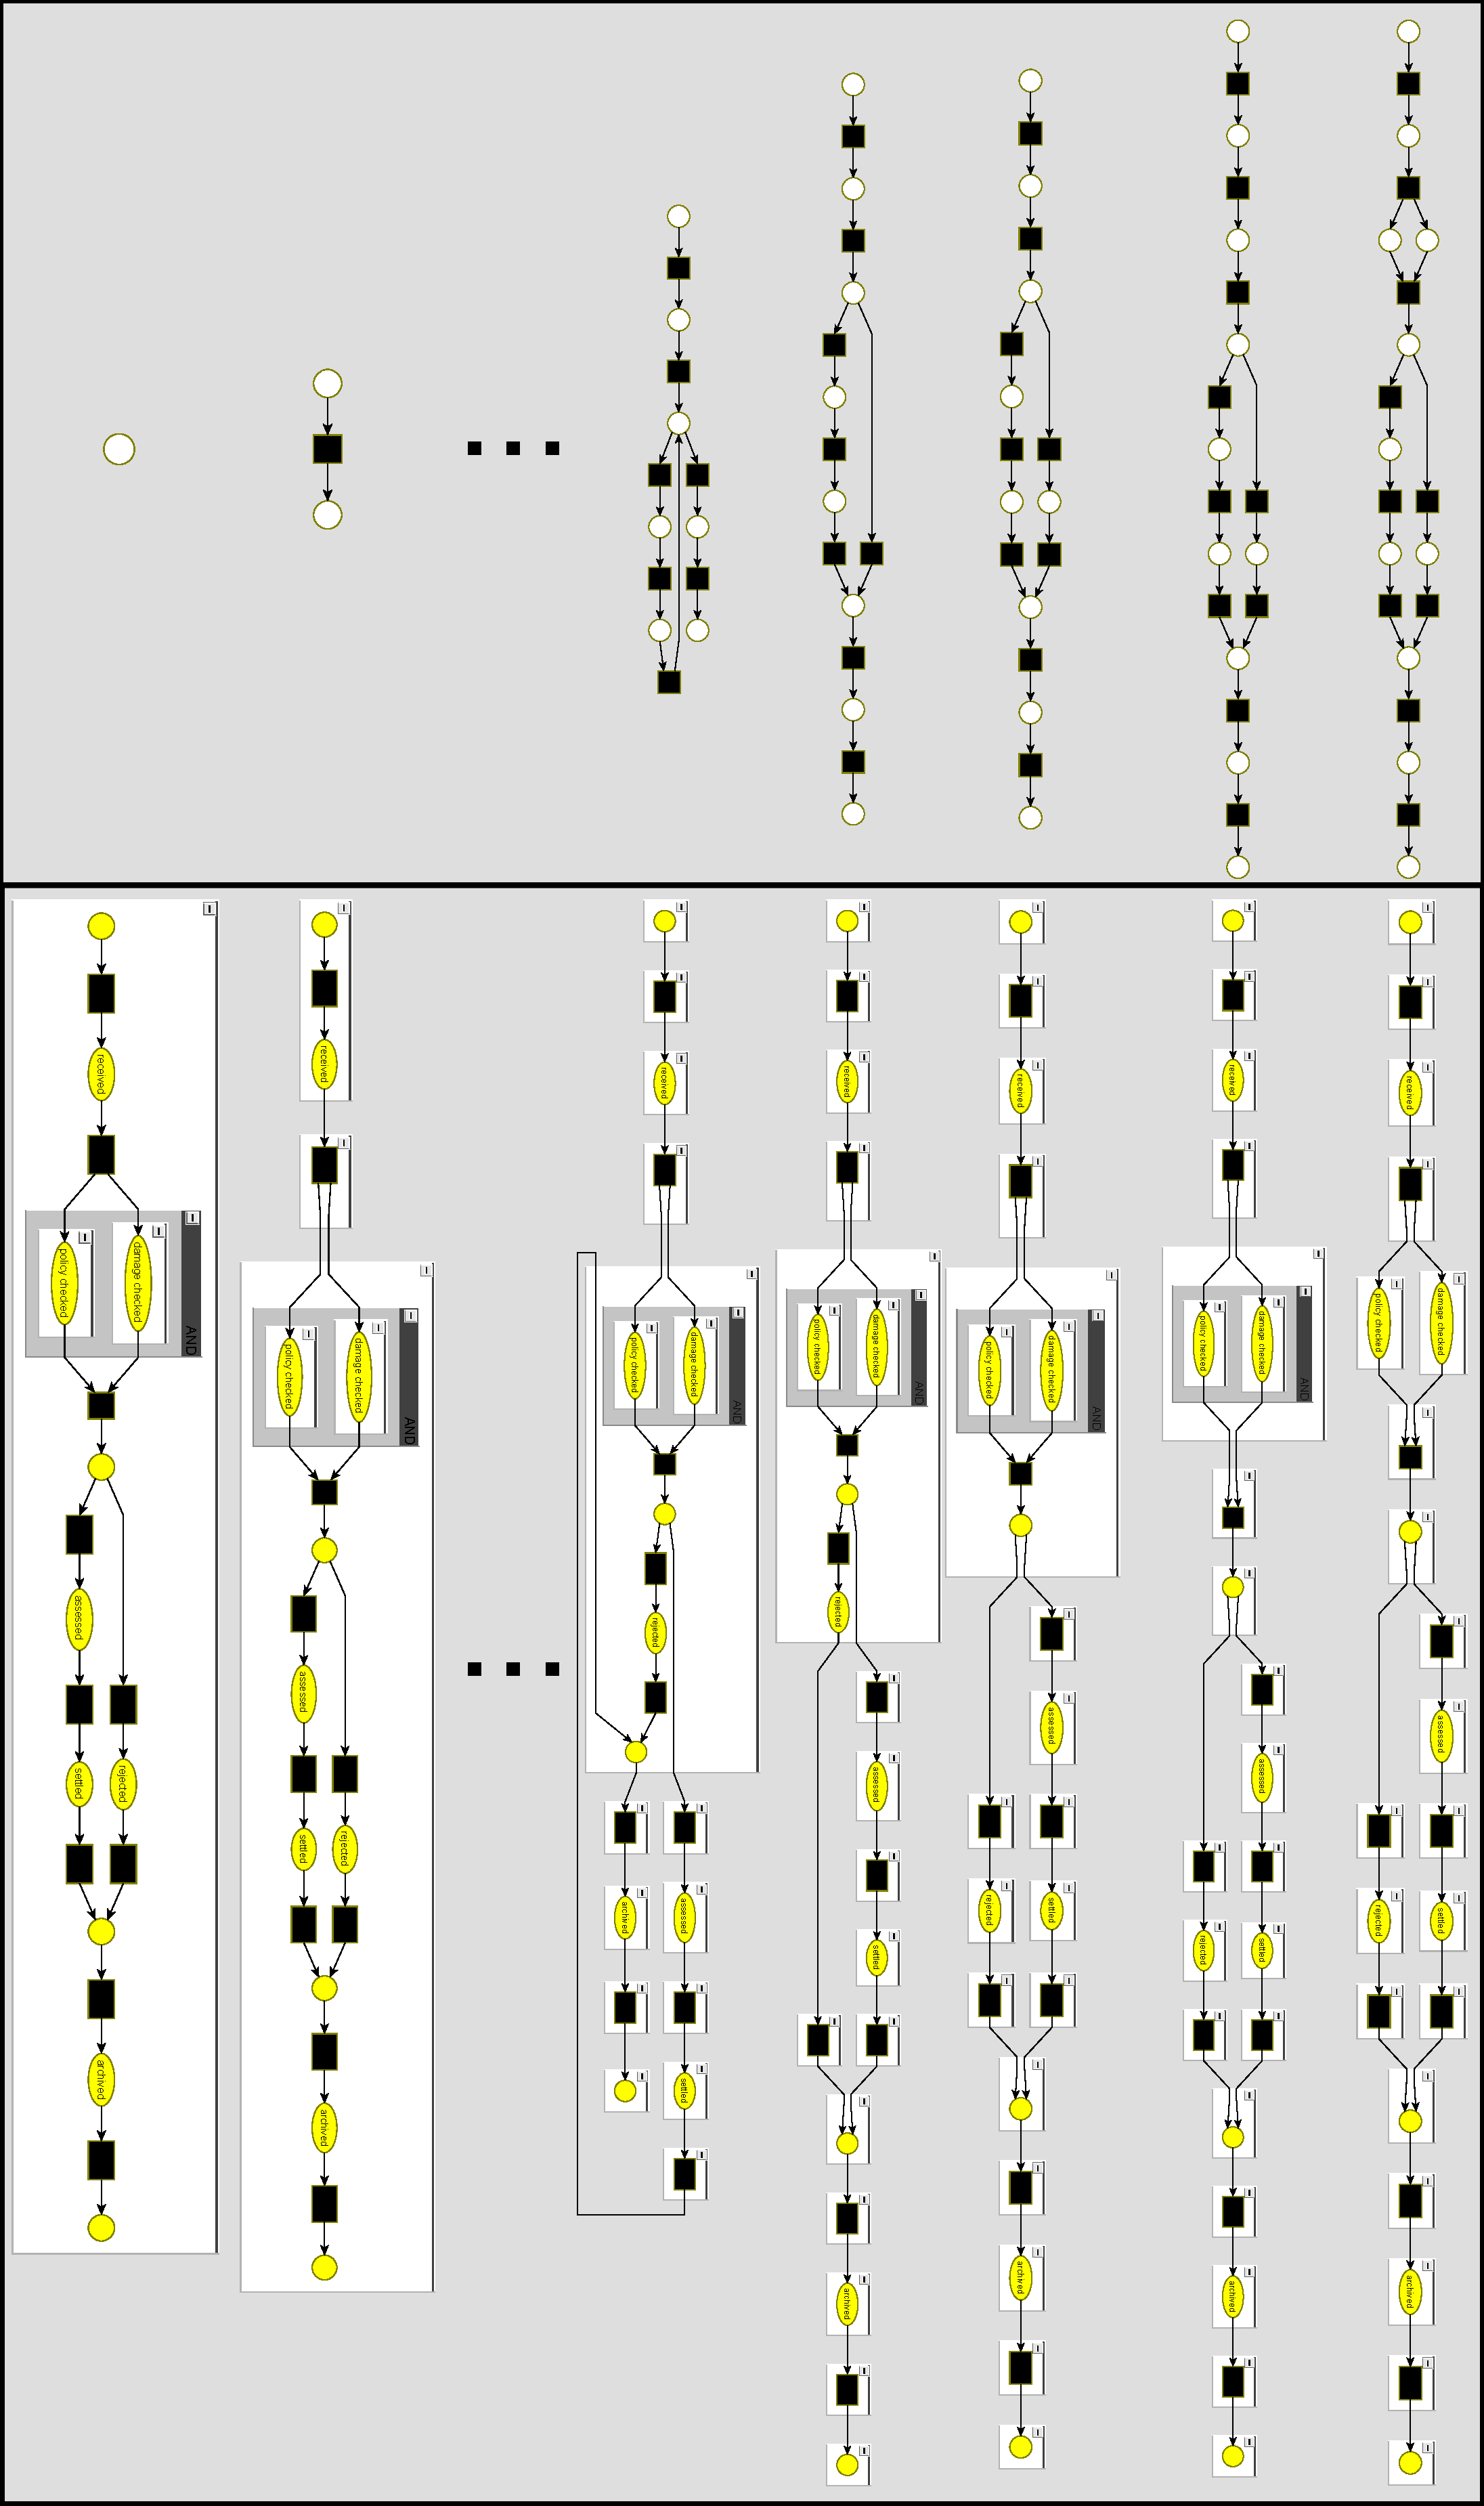
\includegraphics[height=0.8\paperheight]{images/sequence-trim}
\par\end{centering}

\caption{\label{fig:Visualization-ANDandOR}Visualization of an execution trace
of the AND and OR reduction rules.}


\end{figure}


The figure shows downwards subsequent applications of reduction rules.
The second to fifth snapshots are the result of applying in sequence
once the AND rule and three times the OR rule. From the figure it
cannot be determined which variant of the AND rule has been applied
in the first step since they would both lead to the second snapshot
in Figure~\ref{fig:Visualization-ANDandOR} The bottom of the figure
shows a final application of the OR rule. Since the final snapshot
contains exactly one input place, the output statechart can be considered
valid. The details of embedding the final structure in a StateChart
container element are straightforward and not shown in Figure~\ref{fig:Visualization-ANDandOR}.


\section{Testsuite and Additional Artifacts}

In this section, we present some testcases that should be used both
for some basic correctness verification as well as for performance
testing. The complete testsuite is available in an online repository%
\footnote{See \url{https://github.com/louismrose/ttc_pn2sc/}%
}. Moreover, we provide online access to additional test materials,
three existing solutions to the case (a Java solution, a GrGen.NET
solution and an Epsilon solution%
\footnote{See \url{http://is.ieis.tue.nl/staff/pvgorp/share/?page=LookupImage&bNameSearch=pn2sc+benchmark}.%
}) and GMF-based editors with automatic layouting features. We will
also participate in online discussions related to these materials
and may submit also improved versions of the existing solutions.


\subsection{Testcase 1: Artificial Example}

\begin{figure}
\begin{centering}
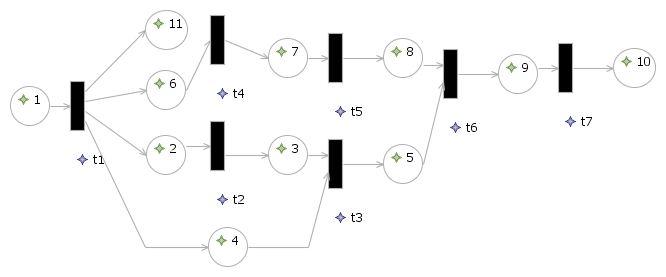
\includegraphics[width=0.6\linewidth]{images/paper-example-pn}
\par\end{centering}

\caption{\label{fig:Testcase-1}Testcase 1 input, diagram exported from a GMF-based
Petri-Net editor.}


\end{figure}


\begin{figure}
\begin{centering}
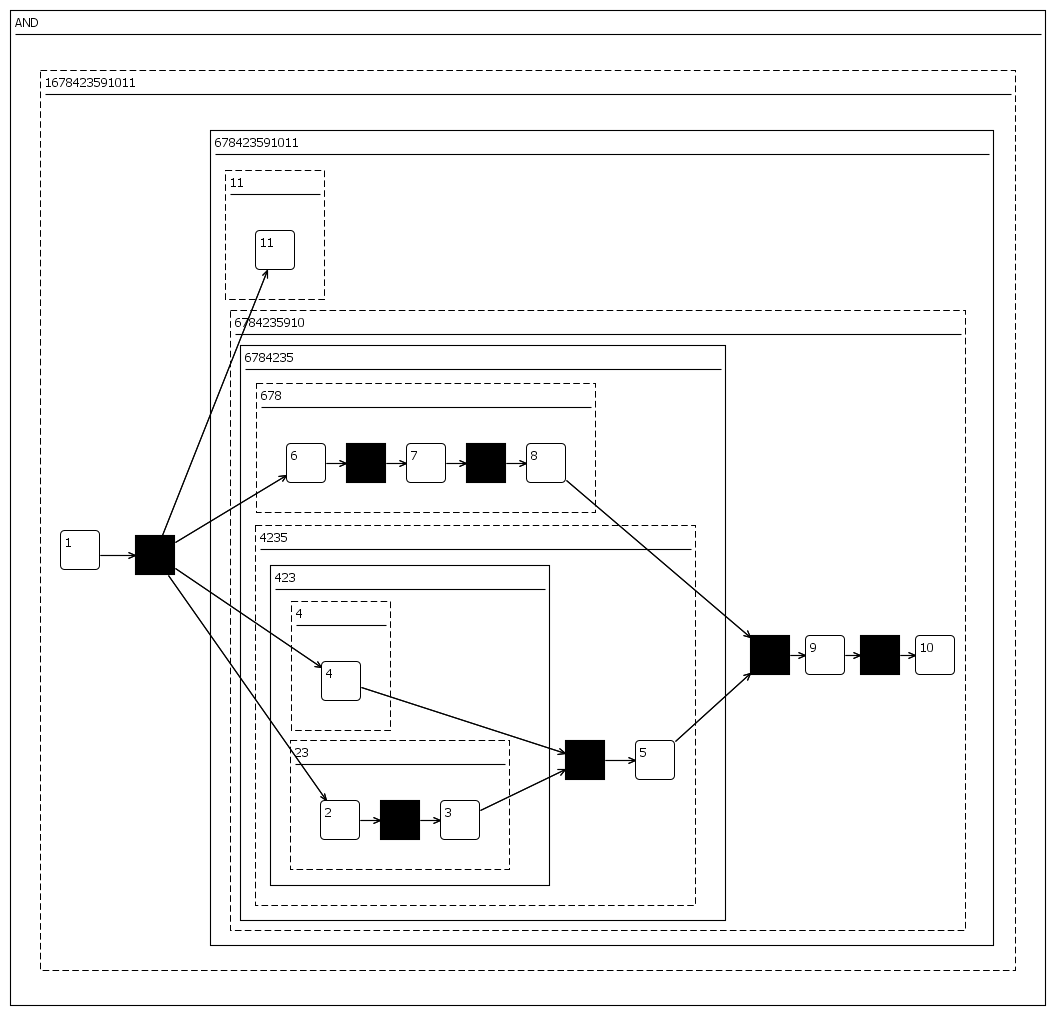
\includegraphics[width=1\linewidth]{images/paper-example-sc}
\par\end{centering}

\caption{\label{fig:Testcase-1-1}Testcase 1 output, diagram exported from
a GMF-based Statechart editor.}
\end{figure}



\section{Evaluation Criteria}


\subsection{Basic Criteria}


\subsection{Bonus Criteria}

- ability to formalize safe net class and (semi-)automatically proof
that reduction rules indeed terminate for that class.

- ability to use a petri-net simulator for simulating the statechart,
or vice versa (note: need simple Token extension to MM)

- rule extension: modular extension to rules for dealing with cross-synchronization


\section{Format for Presenting Evaluation Results}

Table~XXX provides an overview of key characteristics of the three
existing solutions to the case. TODO: explain why these aspects, TODO:
add performance results

\vspace{5mm}
 \textbf{Acknowledgements}: The authors thank Prof. Juan de Lara for
constructing the initial versions of the Petri-Net and statecharts
metamodels used in this case.

\bibliographystyle{plain}
\bibliography{pn2sc}
 \bibliographystyle{eptcs}
\end{document}
